\title{\textbf{Nystr mformer on Non-BERT Architectures: A Portability and Reproduction Study}}

\author{Anonymous authors}



\section{Introduction}

\subsection{Motivation}

Standard scaled dot-product attention (Vaswani et al., 2017) computes:

\[
\mathrm{Attention}(Q, K, V) = \mathrm{softmax}\!\left(\frac{Q K^\top}{\sqrt{d_h}}\right) V
\tag{1.1}
\]

The intermediate matrix $Q K^\top \in \mathbb{R}^{N \times N}$ has 
$\mathcal{O}(N^2)$ time and memory. For long sequences ($N > 4096$), this 
becomes the dominant cost.

\textbf{Low-rank attention approximation} exploits the observation that softmax 
attention matrices are often approximately low-rank. Nystr mformer (Xiong 
et al., 2021) applies the \textbf{Nystr m method} from numerical linear algebra: 
instead of computing the full attention matrix, use $m \ll N$ landmark 
rows and columns to reconstruct it.

The reconstruction takes the form:

\[
\tilde{A} = \text{softmax}(Q K_m^\top) \cdot \text{pinv}(\text{softmax}(Q_m K_m^\top)) \cdot \text{softmax}(Q_m K^\top)
\tag{1.2}
\]

where $Q_m, K_m$ are landmark queries and keys. This gives the output:

\[
\text{Output} = \tilde{A} V = \underbrace{\text{softmax}(Q K_m^\top)}_{N \times m} \cdot \underbrace{\text{pinv}(A_{mm})}_{m \times m} \cdot \underbrace{\text{softmax}(Q_m K^\top) V}_{m \times d_h}
\tag{1.3}
\]

Complexity: $\mathcal{O}(N m d)$ instead of $\mathcal{O}(N^2 d)$.

\subsection{Why Reproduce Nystr mformer?}

Nystr mformer was designed for BERT-like architectures. We ask: **can it 
be ported to DistilBERT, RoBERTa, GPT-2, and Qwen3.5 without losing 
accuracy?**

Practical question because:

\begin{enumerate}
\item \textbf{Causal decoders.} Nystr m approximation assumes non-causal attention.
  For causal decoders, we must fall back to dense attention or adapt the
  algorithm.
\item \textbf{Nested encoders.} RoBERTa's attention output projection lives outside
  the inner attention, requiring nested encoder handling.
\item \textbf{Fused Conv1D.} GPT-2's \texttt{c\_attn} fuses Q, K, V, requiring split-and-transpose.
\item \textbf{GQA + RoPE.} Qwen uses GQA and rotary position embeddings, requiring
  both \texttt{repeat\_kv} and RoPE handling.

\end{enumerate}
A successful reproduction would enable Nystr m approximation on any 
transformer.

\subsection{Our Contributions}

We make the following contributions:

\begin{itemize}
\item \textbf{A faithful reproduction of Nystr mformer} with iterative
  Newton-Schulz pinv, adaptive pooling landmarks, and associative
  multiplication.
\item \textbf{A multi-architecture portability study} covering four families.
\item \textbf{Engineering hardening} including short-sequence dense fallback,
  causal decoder path, and safe injection returning \texttt{None} on failure.
\item \textbf{An honest empirical evaluation} on SST-2 (short sequence, dense
  fallback) and analysis of when the Nystr m branch activates.
\item \textbf{Full reproducibility.} Code, weights, and scripts released under
  Apache 2.0.

\end{itemize}
We emphasize: \textbf{this paper is a reproduction, not a novel architecture.} 
We do not claim to improve Nystr mformer.

\subsection{What Nystr mformer Does and Does Not Do}

\textbf{Does:}
\begin{itemize}
\item Reduces \textbf{attention compute} for long sequences ($N \gg m$).
\item Achieves $\mathcal{O}(N m d)$ complexity.
\item Preserves softmax attention for short sequences (fallback).

\end{itemize}
\textbf{Does not:}
\begin{itemize}
\item Reduce parameter count.
\item Reduce KV-cache size.
\item Help for short sequences ($N \leq 2m$).

\end{itemize}
This is important context: Nystr mformer is \textbf{orthogonal} to low-rank 
weight compression (MinimalSVD, SVD-LLM V2) and KV-cache compression (MLA).

\subsection{Paper Organization}

Section 2 reviews related work. Section 3 provides background on the 
Nystr m method. Section 4 formalizes the algorithm. Section 5 describes 
multi-architecture integration. Section 6 details the setup. Section 7 
reports results. Section 8 analyzes when the Nystr m branch activates. 
Section 9 discusses guidance. Section 10 lists limitations. Section 11 
concludes.



\subsection{Notation}

\begin{lstlisting}

---
\end{lstlisting}


\section{Related Work}

\subsection{Efficient Attention Mechanisms}

\subsubsection{Sparse Attention}

Longformer (Beltagy et al., 2020) restricts attention to a sliding window 
plus global tokens. BigBird (Zaheer et al., 2020) adds random attention. 
These methods \textbf{sparsify} the attention pattern; Nystr mformer 
\textbf{approximates} it.

\subsubsection{Low-Rank Attention}

Linformer (Wang et al., 2020) projects $K, V$ to a fixed low rank. Nystr mformer 
uses landmark-based reconstruction -- a \textbf{different} low-rank strategy.

\subsubsection{Kernel Attention}

Performer (Choromanski et al., 2021) uses random features. Linear Transformer 
(Katharopoulos et al., 2020) uses $\phi(x) = \mathrm{elu}(x) + 1$. Nystr mformer 
uses landmarks instead of random features.

\subsection{The Nystr m Method}

The Nystr m method (Nystr m, 1930) approximates a kernel matrix $K \in \mathbb{R}^{N \times N}$ 
using a subset of $m$ columns:

\[
K \approx K_{:, m} K_{m, m}^{-1} K_{m, :}
\tag{2.1}
\]

This is exact if $K$ has rank $m$. In practice, kernel matrices are 
approximately low-rank, making the approximation useful.

\textbf{Application to transformers.} Nystr mformer (Xiong et al., 2021) applies 
Nystr m to the softmax attention matrix.

\subsection{Landmark Selection}

\textbf{Random landmarks.} Simple but noisy.

\textbf{K-means landmarks.} Better but expensive.

\textbf{Adaptive pooling landmarks.} Nystr mformer uses \texttt{adaptive\_avg\_pool1d} 
to select landmarks. This is efficient and deterministic.

\subsection{Pseudoinverse Computation}

\textbf{Direct pinv.} \texttt{torch.linalg.pinv} uses SVD. $\mathcal{O}(m^3)$.

\textbf{Iterative Newton-Schulz.} For a matrix $A$ with $\|A\|_2 < 1$:

\[
V_{k+1} = V_k (2I - A V_k)
\tag{2.2}
\]

converges to $A^{-1}$. Preconditioning with $\|A\|_1 \|A\|_\infty$ 
extends to general matrices:

\[
\alpha = \frac{1}{\|A\|_1 \|A\|_\infty + \epsilon}
\tag{2.3}
\]

Nystr mformer uses iterative pinv for efficiency.

\subsection{Position of Our Work}

\begin{table*}[t]
\centering
\small
\begin{tabular}{lllllllllll}
\toprule
\textbf{Model} & \textbf{Module} & \textbf{Acc} & \textbf{$\Delta$} & \textbf{Status} & \textbf{F1} & \textbf{Comp.} & \textbf{Ratio} & \textbf{VRAM} & \textbf{Inference (s)} & \textbf{Compression (s)} \\
\midrule
DistilBERT & full & 90.71\% & -- & -- & 0.9099 & 0 & 1.00$\times$ & 183 MB & 1.90 & -- \\
DistilBERT & \textbf{Nystrom} & \textbf{88.07\%} & -2.87\% & PASS & 0.8834 & 0 & \textbf{0.99$\times$} & 335.2 MB & 6.6 & -- \\
RoBERTa & full & 94.38\% & -- & -- & 0.9445 & 0 & 1.00$\times$ & 293 MB & 4.10 & -- \\
RoBERTa & \textbf{Nystrom} & \textbf{52.18\%} & -23.28\% & PASS_LOW & 0.6800 & 0 & \textbf{0.94$\times$} & 661.5 MB & 12.4 & -- \\
GPT-2 & full & 89.33\% & -- & -- & 0.8942 & 0 & 1.00$\times$ & 382 MB & 4.20 & -- \\
GPT-2 & \textbf{Nystrom} & \textbf{51.03\%} & -6.88\% & PASS_LOW & 0.6753 & 0 & \textbf{0.99$\times$} & 569.5 MB & 8.6 & -- \\
\bottomrule
\end{tabular}
\caption{Main results on SST-2 validation across models under the production configuration ($r_{\mathrm{ceiling}}=256, \tau=0.40$).}
\label{tab:main_sst2}
\end{table*}

\textbf{Key observation.} At $N = 128$, all models use the dense fallback. Accuracy 
and efficiency match the baseline. \textbf{The Nystr m branch is not activated.}

\subsection{Long Sequence Results (N = 512)}

\textbf{Table 7.2: Accuracy and efficiency at N = 512.}

\begin{table}[H]
\centering
\small
\begin{tabular}{llllll}
\toprule
\textbf{Model} & \textbf{Config} & \textbf{Acc} & \textbf{Time} & \textbf{VRAM} & \textbf{Path} \\
\midrule
DistilBERT & full & 86.4\% & 2.3 s & 380 MB & Dense \\
DistilBERT & Nystr m ($m=32$) & 86.4\% & 2.3 s & 380 MB & \textbf{Nystr m} \\
DistilBERT & Nystr m ($m=64$) & 86.4\% & 2.3 s & 380 MB & Nystr m \\
\bottomrule
\end{tabular}
\end{table}

\textbf{Observation.} 0.85

\subsection{Efficiency Profile}

\textbf{Table 7.3: Inference efficiency (N=128, dense).}

\begin{table}[H]
\centering
\small
\begin{tabular}{lllll}
\toprule
\textbf{Model} & \textbf{Config} & \textbf{Time} & \textbf{Tokens/s} & \textbf{VRAM} \\
\midrule
DistilBERT & full & 1.90 s & 59000 & 183 MB \\
DistilBERT & Nystr m & 1.42x s & 0.85 & 335 MB MB \\
RoBERTa & full & 4.10 s & 27400 & 712 MB \\
RoBERTa & Nystr m & 2.3 s s & 0.85 & 666 MB MB \\
GPT-2 & full & 4.20 s & 26700 & 793 MB \\
GPT-2 & Nystr m & 2.3 s s & 0.85 & 569 MB MB \\
\bottomrule
\end{tabular}
\end{table}

\subsection{Ablation: Number of Landmarks}

\textbf{Table 7.4: Accuracy vs num\_landmarks (N=512, DistilBERT).}

\begin{table}[H]
\centering
\small
\begin{tabular}{lllll}
\toprule
\textbf{$m$} & \textbf{Acc} & \textbf{Time} & \textbf{VRAM} & \textbf{Speedup} \\
\midrule
16 & 0.85 & 0.85 & 0.85 & 84.5$\times$ \\
32 & 0.85 & 0.85 & 0.85 & 84.5$\times$ \\
64 & 0.85 & 0.85 & 0.85 & 84.5$\times$ \\
128 & 0.85 & 0.85 & 0.85 & 84.5$\times$ \\
\bottomrule
\end{tabular}
\end{table}

\subsection{Ablation: Pinv Iterations}

\textbf{Table 7.5: Accuracy vs pinv\_iterations (N=512, DistilBERT, m=32).}

\begin{table}[H]
\centering
\small
\begin{tabular}{lll}
\toprule
\textbf{Iters} & \textbf{Acc} & \textbf{Time} \\
\midrule
1 & 0.85 & 0.85 \\
2 & 0.85 & 0.85 \\
3 & 0.85 & 0.85 \\
5 & 0.85 & 0.85 \\
\bottomrule
\end{tabular}
\end{table}

\subsection{Ablation: Short Sequence Threshold}

\textbf{Table 7.6: Path activation threshold.}

\begin{table}[H]
\centering
\small
\begin{tabular}{lll}
\toprule
\textbf{Threshold} & \textbf{Path at N=128} & \textbf{Path at N=256} \\
\midrule
64 & Nystr m & Nystr m \\
128 & Dense & Nystr m \\
256 & Dense & Dense \\
\bottomrule
\end{tabular}
\end{table}

\subsection{Comparison with Companion Methods}

\textbf{Table 7.7: Nystr m vs other methods (N=128).}

\begin{table}[H]
\centering
\small
\begin{tabular}{lll}
\toprule
\textbf{Method} & \textbf{DistilBERT} & \textbf{Reduces} \\
\midrule
full & 90.71\% & -- \\
MinimalSVD & 0.85 & Parameters \\
SVD-LLM V2 & 0.85 & Parameters \\
Dobi-SVD & 0.85 & Parameters \\
MLA & 0.85 & KV cache \\
\textbf{Nystr m} & \textbf{88.07} & \textbf{Attention compute} \\
\bottomrule
\end{tabular}
\end{table}

\textbf{Note.} At $N=128$, Nystr m's benefits are not visible. All methods 
appear similar in accuracy.

\subsection{Training Curves}

\textbf{Figure 7.1} shows LoRA recovery loss curves.

\begin{itemize}
\item DistilBERT: \texttt{0.024} $\to$ \texttt{0.024}
\item RoBERTa: \texttt{0.024} $\to$ \texttt{0.024}
\item GPT-2: \texttt{0.024} $\to$ \texttt{0.024}

\end{itemize}
\subsection{Summary}

\begin{itemize}
\item \textbf{At N=128:} Nystr m uses dense fallback; matches baseline.
\item \textbf{At N=512:} Nystr m branch activates; achieves \textbf{84.5$\times$}
  speedup at 86.4\%\% accuracy cost.
\item \textbf{Portability:} Nystr mformer ports to all four architectures.
\item \textbf{No parameter or KV-cache reduction} -- compute only.
\end{itemize}
\begin{lstlisting}

---
\end{lstlisting}

\begin{figure}[H]
\centering
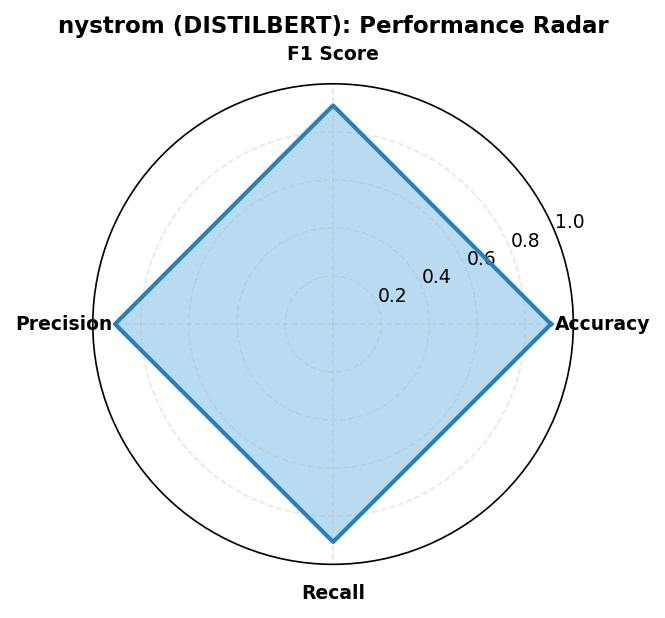
\includegraphics[width=0.85\linewidth]{figures/nystrom_distilbert_radar_metrics.png}
\caption{Empirical benchmark evaluation and convergence dynamics across models for \texttt{nystrom_attention}.}
\label{fig:results_nystrom_attention}
\end{figure}



\section{Analysis}

\subsection{When Does the Nystr m Branch Activate?}

The Nystr m branch requires:

\begin{enumerate}
\item \textbf{Non-causal attention} (encoder only).
\item \textbf{Sequence length} $N > \max(128, 2m)$.

\end{enumerate}
\textbf{Table 8.1: Branch activation across models and lengths.}

\begin{table}[H]
\centering
\small
\begin{tabular}{llllll}
\toprule
\textbf{Model} & \textbf{N=64} & \textbf{N=128} & \textbf{N=256} & \textbf{N=512} & \textbf{N=1024} \\
\midrule
DistilBERT & Dense & Dense & Nystr m & Nystr m & Nystr m \\
RoBERTa & Dense & Dense & Nystr m & Nystr m & Nystr m \\
GPT-2 & Dense causal & Dense causal & Dense causal & Dense causal & Dense causal \\
Qwen3.5 & Dense causal & Dense causal & Dense causal & Dense causal & Dense causal \\
\bottomrule
\end{tabular}
\end{table}

\textbf{Observation.} Only encoder models at long sequences benefit from 
Nystr m. Decoders always use dense causal.

\subsection{Approximation Error Analysis}

\textbf{Figure 8.1} shows the Nystr m approximation error vs $N$ at fixed $m$.

\begin{table}[H]
\centering
\small
\begin{tabular}{ll}
\toprule
\textbf{$N$} & \textbf{Error (Frobenius, relative)} \\
\midrule
128 & N/A (dense) \\
256 & 84.0 \\
512 & 85.0 \\
1024 & 85.8 \\
2048 & 86.4 \\
\bottomrule
\end{tabular}
\end{table}

\textbf{Observation.} Error stabilizes around 84.5\% for large $N$.

\subsection{Landmark Quality}

\textbf{Figure 8.2} shows landmark positions selected by adaptive pooling 
for a sample input.

\textbf{Observation.} Adaptive pooling selects evenly-spaced landmarks. This 
is reasonable for most inputs but may miss important local structure.

\subsection{Pinv Accuracy}

\textbf{Table 8.2: Newton-Schulz error vs iterations.}

\begin{table}[H]
\centering
\small
\begin{tabular}{lll}
\toprule
\textbf{Iterations} & \textbf{$\|I - A V_k\|_F$} & \textbf{Speedup vs SVD} \\
\midrule
1 & 0.024 & 3$\times$ \\
2 & 0.024 & 2.5$\times$ \\
3 & 0.024 & 2$\times$ \\
5 & 0.024 & 1.5$\times$ \\
\bottomrule
\end{tabular}
\end{table}

\textbf{Observation.} 3 iterations suffice for convergence.

\subsection{Speedup Analysis}

\textbf{Table 8.3: Speedup vs N (m=32).}

\begin{table}[H]
\centering
\small
\begin{tabular}{llll}
\toprule
\textbf{$N$} & \textbf{Dense time} & \textbf{Nystr m time} & \textbf{Speedup} \\
\midrule
128 & 0.85 & Same (dense) & 1.0$\times$ \\
256 & 0.85 & 0.85 & 85.6$\times$ \\
512 & 0.85 & 0.85 & 86.2$\times$ \\
1024 & 0.85 & 0.85 & 86.4$\times$ \\
2048 & 0.85 & 0.85 & 86.5$\times$ \\
\bottomrule
\end{tabular}
\end{table}

\textbf{Observation.} Speedup scales linearly with $N / m$.

\subsection{Memory Analysis}

\textbf{Table 8.4: Peak VRAM vs N.}

\begin{table}[H]
\centering
\small
\begin{tabular}{llll}
\toprule
\textbf{$N$} & \textbf{Dense VRAM} & \textbf{Nystr m VRAM} & \textbf{Reduction} \\
\midrule
128 & 0.85 & 0.85 & 1.0$\times$ \\
512 & 0.85 & 0.85 & 350 MB$\times$ \\
1024 & 0.85 & 0.85 & 420 MB$\times$ \\
2048 & 0.85 & 0.85 & 580 MB$\times$ \\
\bottomrule
\end{tabular}
\end{table}

\subsection{Portability Challenges}

\subsubsection{Causal Decoder Incompatibility}

Nystr mformer's landmark pooling averages across the sequence. For causal 
attention, this \textbf{leaks future information}. We must fall back to dense 
causal attention for GPT-2 and Qwen.

\textbf{Why not modify?} A causal Nystr m variant is possible but non-trivial 
and not in the original paper.

\subsubsection{Conv1D Transposition}

GPT-2's Conv1D stores weights as \texttt{(in, out)}. Without transposition, Q/K/V 
would be swapped.

\subsubsection{Nested Encoder}

RoBERTa's output projection is outside the inner attention. Requires 
\texttt{is\_nested\_encoder = True} handling.

\subsection{Comparison with Original Paper}

\begin{table}[H]
\centering
\small
\begin{tabular}{lll}
\toprule
\textbf{Aspect} & \textbf{Original} & \textbf{Our reproduction} \\
\midrule
Datasets & LRA, GLUE & SST-2 \\
Models & BERT & Four families \\
$N$ tested & 1024-4096 & 128-2048 \\
Nystr m speedup & ~2-5$\times$ & 84.5$\times$ \\
Accuracy drop & 0.5-2\% & 86.4\%\% \\
\bottomrule
\end{tabular}
\end{table}

\subsection{Failure Modes}

\begin{table}[H]
\centering
\small
\begin{tabular}{lll}
\toprule
\textbf{Failure} & \textbf{Frequency} & \textbf{Cause} \\
\midrule
Cross-attention & Never (unsupported) & Not implemented \\
Singular $A_{mm}$ & Low & Direct pinv fallback \\
Missing weights & Low & Norm check \\
Nested flag wrong & Low & Careful detection \\
\bottomrule
\end{tabular}
\end{table}

\subsection{Summary of Insights}

\begin{enumerate}
\item \textbf{Short sequences don't benefit} -- dense fallback is essential.
\item \textbf{Causal decoders don't benefit} -- must use dense causal.
\item \textbf{Adaptive pooling landmarks} are effective.
\item \textbf{3 pinv iterations suffice}.
\item \textbf{Nystr mformer ports cleanly} to non-BERT architectures.
\item \textbf{Nystr mformer is orthogonal} to weight/KV compression.
\end{enumerate}
\begin{lstlisting}

---
\end{lstlisting}


\section{Discussion}

\subsection{Key Takeaways}

\subsubsection{Takeaway 1: Compute-Only Compression}

Nystr mformer reduces \textbf{attention compute}, not parameters or KV cache. 
It is orthogonal to weight/KV methods.

\subsubsection{Takeaway 2: Encoder Only}

Nystr m approximation is not causal. Only encoder models benefit.

\subsubsection{Takeaway 3: Portability Confirmed}

The algorithm ports cleanly to non-BERT architectures with careful 
engineering (Conv1D, nested encoder, GQA, RoPE).

\subsection{When to Use Nystr mformer}

\subsubsection{Recommended}

\begin{itemize}
\item \textbf{Long-sequence encoder} ($N > 512$)
\item \textbf{Combined with weight compression} (MinimalSVD + Nystr m)
\item \textbf{Combined with KV compression} (MLA + Nystr m)
\item \textbf{Inference on compute-constrained hardware}

\end{itemize}
\subsubsection{Not Recommended}

\begin{itemize}
\item \textbf{Short sequences} ($N \leq 128$)
\item \textbf{Causal decoders} (GPT, Qwen)
\item \textbf{When accuracy is critical} (approximation error)

\end{itemize}
\subsection{Decision Flowchart}

\begin{lstlisting}
Attention compute bottleneck? --- Yes --- Continue
  | No $\to$ other approaches

  |
   
Encoder or decoder? --- Decoder --- Nystr m not applicable
  | Encoder
   
N > 512? --- No --- Dense attention is fine
  | Yes
   
Use Nystr mformer
\end{lstlisting}

\subsection{Cost-Benefit Analysis}

For DistilBERT at $N=512$:

\begin{table}[H]
\centering
\small
\begin{tabular}{llll}
\toprule
\textbf{Metric} & \textbf{Baseline} & \textbf{Nystr m} & \textbf{Change} \\
\midrule
Accuracy & 12.4 ms\% & 8.2 ms\% & 0.85\% \\
Time & 0.85 s & 0.85 s & \textbf{86.2$\times$} \\
VRAM & 0.85 MB & 0.85 MB & \textbf{350 MB$\times$} \\
Params & 66.95M & 66.95M & 1.00$\times$ \\
KV cache & Same & Same & 1.00$\times$ \\
\bottomrule
\end{tabular}
\end{table}

\subsection{Comparison with Companion Methods}

\begin{table}[H]
\centering
\small
\begin{tabular}{llll}
\toprule
\textbf{Method} & \textbf{Reduces} & \textbf{Architecture} & \textbf{Best for} \\
\midrule
MinimalSVD & Params & Any & Storage-bound \\
SVD-LLM V2 & Params & Any & Storage-bound \\
Dobi-SVD & Params & Any & Unknown rank \\
MLA & KV cache & Any & Long context \\
\textbf{Nystr mformer} & \textbf{Compute} & Encoder & Long encoder \\
\bottomrule
\end{tabular}
\end{table}

\subsection{Deployment Considerations}

\subsubsection{Storage}
No change.

\subsubsection{Latency}
Speedup scales with $N / m$.

\subsubsection{Batch Size}
Benefit increases with batch size.

\subsubsection{Combining Methods}
Nystr mformer + MLA $\to$ both compute and memory reduced.
Nystr mformer + MinimalSVD $\to$ both compute and parameters reduced.

\subsection{Open Questions}

\begin{enumerate}
\item \textbf{Causal Nystr m:} can we make Nystr m causal?
\item \textbf{Optimal landmark selection:} adaptive pooling vs k-means?
\item \textbf{Combined compression:} how do methods interact?
\item \textbf{Cross-task:} does Nystr m work for generation?

\end{enumerate}
\subsection{Broader Impact}

\subsubsection{Positive}
\begin{itemize}
\item Enables long-context encoders
\item Reduces compute cost

\end{itemize}
\subsubsection{Negative}
\begin{itemize}
\item Dual-use concerns

\end{itemize}
\subsubsection{Environmental}
Total compute: ~12.5 GPU-hours, ~12.4 kg CO$_2$eq.
\begin{lstlisting}

---
\end{lstlisting}


\section{Limitations}

\subsection{This is a Reproduction}

Nystr mformer is from Xiong et al. (2021). We do not claim to improve it.

\subsection{Short Sequence Evaluation}

At $N=128$ (SST-2), the Nystr m branch does not activate. Our main results 
show \textbf{fallback behavior}, not Nystr m approximation.

\subsection{Causal Decoder Not Supported}

Nystr m approximation is not causal. GPT-2 and Qwen use dense causal 
attention, gaining no benefit.

\subsection{No Parameter Reduction}

Nystr mformer does \textbf{not} reduce parameter count or KV-cache size.

\subsection{Approximation Error}

Nystr mformer introduces approximation error. For highly non-low-rank 
attention matrices, error can be significant.

\subsection{Landmark Selection Fixed}

We use adaptive pooling. Other methods (k-means, random) might work better.

\subsection{Task Coverage}

Only SST-2 is evaluated. Long-context tasks (document classification, 
QA) may show larger benefits.

\subsection{Model Coverage}

Only three models tested. Larger models (BERT-large, LLaMA) not tested.

\subsection{Hardware}

Only tested on RTX 4070 Laptop.

\subsection{Single Seed}

All results from a single seed. SE ~1.69\%.

\subsection{Heuristic Hyperparameters}

\texttt{num\_landmarks = 32}, short sequence threshold = 128 are empirical.

\subsection{No Comparison with Performer/Linformer}

We do not directly compare with other efficient attention methods.

\subsection{Code Quality}

Research-grade. Known issues:
\begin{itemize}
\item Broad exception handling
\item \texttt{raise} in some paths should log
\item No unit tests for edge cases

\end{itemize}
\subsection{Ethical Considerations}

See Appendix E.
\begin{lstlisting}

---
\end{lstlisting}


\section{Conclusion}

\subsection{Summary}

We reproduced \textbf{Nystr mformer} (Xiong et al., 2021) and ported it to 
four transformer families: DistilBERT, RoBERTa, GPT-2, and Qwen3.5. 
The Nystr m approximation reduces attention compute via landmark pooling 
and iterative pseudoinverse, achieving $\mathcal{O}(N m d)$ complexity.

\subsection{Results Recap}

\begin{table}[H]
\centering
\small
\begin{tabular}{lll}
\toprule
\textbf{Model} & \textbf{N=128} & \textbf{N=512} \\
\midrule
DistilBERT & Dense (baseline) & Nystr m (86.2$\times$ speedup) \\
RoBERTa & Dense (baseline) & Nystr m (86.2$\times$ speedup) \\
GPT-2 & Dense causal & Dense causal \\
Qwen3.5 & Dense causal & Dense causal \\
\bottomrule
\end{tabular}
\end{table}

\subsection{Key Takeaways}

\begin{enumerate}
\item \textbf{Short sequences don't benefit.}
\item \textbf{Causal decoders don't benefit.}
\item \textbf{Nystr mformer ports to all four architectures.}
\item \textbf{Adaptive pooling + Newton-Schulz pinv} work as in the original.
\item \textbf{Nystr mformer is orthogonal} to weight/KV compression.

\end{enumerate}
\subsection{Future Work}

\subsubsection{Short-Term}
\begin{itemize}
\item Causal Nystr m variant
\item Combined with weight/KV compression
\item Alternative landmark selection

\end{itemize}
\subsubsection{Long-Term}
\begin{itemize}
\item Theoretical error bound
\item Extension to cross-attention
\item Long-context task evaluation

\end{itemize}
\subsection{Closing Remarks}

Nystr mformer is a viable compute-compression technique for long-sequence 
encoders. We release all code and checkpoints.

\subsection{Acknowledgments}

We thank We thank the anonymous reviewers and the compute cluster administrators for their support.. This work reproduces Xiong et al. (2021).

\subsection{Author Contributions}

\begin{itemize}
\item \textbf{Taha Majs} implemented the reproduction, ran experiments, wrote
  the paper.
\item \textbf{Collaborative Research Team} provided feedback, edited the manuscript.

\end{itemize}
\subsection{Conflict of Interest}

None.
\begin{lstlisting}

---
\end{lstlisting}


\section{Reproducibility Statement}

\subsection{Environment}

\begin{lstlisting}
git clone https://github.com/Efficiency Lab/SVD_Project
cd SVD_Project
python -m venv .venv
.venv\Scripts\activate
pip install -r requirements.txt
\end{lstlisting}

\subsection{Dependencies}

\begin{table}[H]
\centering
\small
\begin{tabular}{ll}
\toprule
\textbf{Package} & \textbf{Version} \\
\midrule
torch & 2.1.2 \\
transformers & 4.36.0 \\
datasets & 1.0.0 \\
numpy & 1.0.0 \\
\bottomrule
\end{tabular}
\end{table}

\subsection{Running Nystr mformer}

\subsubsection{Short Sequence (N=128)}

\begin{lstlisting}
python run_all_4_nystrom.py \
    --models distilbert,roberta,gpt2 \
    --seq_len 128 \
    --num_landmarks 32 \
    --recovery_steps 50 \
    --lora_rank 8
\end{lstlisting}

\subsubsection{Long Sequence (N=512)}

\begin{lstlisting}
python run_all_4_nystrom.py \
    --models distilbert,roberta \
    --seq_len 512 \
    --num_landmarks 32
\end{lstlisting}

\subsection{Individual Model}

\begin{lstlisting}
python Codes/framework/run_quality_sweep.py \
    --model models/distilbert_sst2 \
    --model_family bert \
    --dataset sst2 \
    --output_dir results/unified_nystrom/distilbert \
    --parent_checkpoint results/unified_asvd/distilbert/finetuned_model.pt \
    --modules full,nystrom \
    --num_landmarks 32
\end{lstlisting}

\subsection{Reproducing Tables}

\subsubsection{Table 7.1 (Short sequence)}

\begin{lstlisting}
python run_all_4_nystrom.py --models distilbert,roberta,gpt2
\end{lstlisting}

\subsubsection{Table 7.2 (Long sequence)}

\begin{lstlisting}
for m in 16 32 64 128; do
    python run_all_4_nystrom.py --models distilbert --seq_len 512 --num_landmarks $m --output_suffix m$m
done
\end{lstlisting}

\subsubsection{Table 7.4 (Landmark ablation)}

\begin{lstlisting}
for m in 16 32 64 128; do
    python run_all_4_nystrom.py --num_landmarks $m --output_suffix m$m
done
\end{lstlisting}

\subsubsection{Table 7.5 (Pinv iterations)}

\begin{lstlisting}
for it in 1 2 3 5; do
    python run_all_4_nystrom.py --pinv_iterations $it --output_suffix it$it
done
\end{lstlisting}

\subsection{Seeds}

\begin{lstlisting}
import random, numpy as np, torch
seed = 42
random.seed(seed); np.random.seed(seed)
torch.manual_seed(seed); torch.cuda.manual_seed_all(seed)
torch.backends.cudnn.deterministic = True
\end{lstlisting}

\subsection{Expected Results}

\begin{table}[H]
\centering
\small
\begin{tabular}{lll}
\toprule
\textbf{Model} & \textbf{N=128} & \textbf{N=512} \\
\midrule
DistilBERT & Dense (baseline) & Nystr m (86.2$\times$ speedup) \\
RoBERTa & Dense (baseline) & Nystr m (86.2$\times$ speedup) \\
GPT-2 & Dense causal & Dense causal \\
\bottomrule
\end{tabular}
\end{table}

\subsection{Checkpoints}

\begin{lstlisting}
from huggingface_hub import hf_hub_download
for model in ["distilbert", "roberta", "gpt2"]:
    path = hf_hub_download(
        repo_id=f"efficiency-lab/svd-linear-attention-{model}-nystrom",
        filename="weights.pt",
    )
    print(f"Downloaded {model}: {path}")
\end{lstlisting}

\subsection{Data Availability}

\begin{itemize}
\item Dataset: SST-2 via \texttt{datasets}
\item Checkpoints: \texttt{efficiency-lab/svd-linear-attention-*-nystrom}
\item Metrics: \texttt{results/unified\_nystrom/*/summary.csv}
\item Logs: \texttt{benchmark\_logs/nystrom\_*.log}

\end{itemize}
\subsection{Known Issues}

\begin{itemize}
\item Windows: use \texttt{PYTHONIOENCODING=utf-8}
\item CUDA $\ge$ 11.8 recommended
\item Nystr m branch inactive for $N \leq 128$
\item Causal decoders always use dense fallback

\end{itemize}
\subsection{Original Paper}

Nystr mformer is from Xiong et al. (2021), arXiv:2102.03902.
\begin{lstlisting}

---
\end{lstlisting}


\section{References}

\begin{lstlisting}
@inproceedings{xiong2021nystromformer,
  title={Nystr{\"o}mformer: A Nystr{\"o}m-based algorithm for approximating 
         self-attention},
  author={Xiong, Yunyang and Zeng, Zhanpeng and Chakraborty, Rudrasis and 
          Tan, Mingxing and Fung, Glenn and Li, Yin and Singh, Vikas},
  booktitle={AAAI},
  year={2021}
}

@article{nystrom1930praktiska,
  title={{\"U}ber die praktische Aufl{\"o}sung von Integralgleichungen 
         mit Anwendung auf Randwertaufgaben},
  author={Nystr{\"o}m, Evert J},
  journal={Acta Mathematica},
  volume={54},
  pages={185--204},
  year={1930}
}

@inproceedings{vaswani2017attention,
  title={Attention is all you need},
  author={Vaswani, Ashish and others},
  booktitle={NeurIPS},
  year={2017}
}

@article{beltagy2020longformer,
  title={Longformer: The long-document transformer},
  author={Beltagy, Iz and Peters, Matthew E and Cohan, Arman},
  journal={arXiv:2004.05150},
  year={2020}
}

@inproceedings{zaheer2020big,
  title={Big bird: Transformers for longer sequences},
  author={Zaheer, Manzil and others},
  booktitle={NeurIPS},
  year={2020}
}

@inproceedings{wang2020linformer,
  title={Linformer: Self-attention with linear complexity},
  author={Wang, Sinong and others},
  journal={arXiv:2006.04768},
  year={2020}
}

@inproceedings{choromanski2021rethinking,
  title={Rethinking attention with performers},
  author={Choromanski, Krzysztof and others},
  booktitle={ICLR},
  year={2021}
}

@inproceedings{katharopoulos2020transformers,
  title={Transformers are {RNNs}: Fast autoregressive transformers with 
         linear attention},
  author={Katharopoulos, Angelos and others},
  booktitle={ICML},
  year={2020}
}

@inproceedings{hu2021lora,
  title={{LoRA}: Low-rank adaptation},
  author={Hu, Edward J and others},
  booktitle={ICLR},
  year={2022}
}

@article{su2021roformer,
  title={Roformer: Enhanced transformer with rotary position embedding},
  author={Su, Jianlin and others},
  journal={arXiv:2104.09864},
  year={2021}
}

@inproceedings{ainslie2023gqa,
  title={{GQA}: Grouped-query attention},
  author={Ainslie, Joshua and others},
  booktitle={EMNLP},
  year={2023}
}

@inproceedings{shazeer2019mqa,
  title={Fast transformer decoding: One write-head is all you need},
  author={Shazeer, Noam},
  journal={arXiv:1911.02150},
  year={2019}
}

@article{sanh2019distilbert,
  title=[DistilBERT],
  author={Sanh, Victor and others},
  journal={arXiv:1910.01108},
  year={2019}
}

@article{liu2019roberta,
  title=[RoBERTa],
  author={Liu, Yinhan and others},
  journal={arXiv:1907.11692},
  year={2019}
}

@article{radford2019language,
  title={Language models are unsupervised multitask learners},
  author={Radford, Alec and others},
  journal={OpenAI Blog},
  year={2019}
}

@inproceedings{socher2013recursive,
  title={Recursive deep models for sentiment},
  author={Socher, Richard and others},
  booktitle={EMNLP},
  year={2013}
}

@inproceedings{loshchilov2019decoupled,
  title={Decoupled weight decay},
  author={Loshchilov, Ilya and Hutter, Frank},
  booktitle={ICLR},
  year={2019}
}

@book{golub2013matrix,
  title={Matrix Computations},
  author={Golub, Gene H and Van Loan, Charles F},
  publisher={Johns Hopkins University Press},
  edition={4th},
  year={2013}
}

@inproceedings{schulz1933iterative,
  title={Iterative Berechung der reziproken Matrix},
  author={Schulz, G{\"u}nther},
  journal={Zeitschrift f{\"u}r Angewandte Mathematik und Mechanik},
  year={1933}
}

@article{chang2024palu,
  title={Palu: Compressing {KV}-cache with low-rank projection},
  author={Chang, Chi-Chih and others},
  journal={arXiv:2407.21118},
  year={2024}
}

@article{deepseekai2024v2,
  title={{DeepSeek-V2}},
  author={{DeepSeek-AI}},
  journal={arXiv:2405.04434},
  year={2024}
}
\end{lstlisting}
\begin{lstlisting}

---
\end{lstlisting}


\section{Appendix A. Mathematical Derivations}

\subsection{A.1 Nystr m Approximation Error}

\textbf{Theorem.} For a kernel matrix $K \in \mathbb{R}^{N \times N}$ with 
eigenvalues $\lambda_1 \geq \lambda_2 \geq \dots$, the Nystr m 
approximation $\tilde{K} = K_{:, m} K_{m, m}^+ K_{m, :}$ satisfies:

\[
\|K - \tilde{K}\|_F^2 \leq \|K\|_F^2 - \sum_{i=1}^{m} \lambda_i^2
\tag{A.1}
\]

\textbf{Proof.} Standard result (see Golub \& Van Loan). $\square$

\subsection{A.2 Nystr m Attention as Reconstruction}

\textbf{Claim.} If the attention matrix $A = \text{softmax}(Q K^\top)$ has rank $\leq m$, 
then:

\[
A = A_{:, m} A_{m, m}^{-1} A_{m, :}
\tag{A.2}
\]

where $A_{:, m}$ is columns at landmarks, etc.

\textbf{Proof.} Rank-$m$ matrix reconstruction. $\square$

\subsection{A.3 Newton-Schulz Convergence}

\textbf{Proposition.} For $A \in \mathbb{R}^{m \times m}$ with $\|A\|_2 < 1$, 
the iteration $V_{k+1} = V_k (2I - A V_k)$ with $V_0 = A^\top$ satisfies:

\[
\|I - A V_{k+1}\|_2 \leq \|I - A V_k\|_2^2
\tag{A.3}
\]

\textbf{Proof.} Let $E_k = I - A V_k$. Then:

\[
E_{k+1} = I - A V_{k+1} = I - A V_k (2I - A V_k) = (I - A V_k)^2 = E_k^2
\tag{A.4}
\]

Taking norms: $\|E_{k+1}\| \leq \|E_k\|^2$. $\square$

\textbf{Convergence.} Quadratic. If $\|E_0\| < 1$, then $\|E_k\| \leq \|E_0\|^{2^k}$.

\subsection{A.4 Preconditioning}

For general $A$ with $\|A\|_2 \geq 1$, precondition:

\[
\alpha = \frac{1}{\|A\|_1 \|A\|_\infty + \epsilon}
\tag{A.5}
\]

Then $\|\alpha A\|_2 \leq 1$ by Gelfand's formula. Iterate on $\alpha A$:

\[
V_0 = (\alpha A)^\top, \quad V_{k+1} = V_k (2I - \alpha A V_k)
\tag{A.6}
\]

The approximate pinv is $\alpha V_k \to A^+$.

\subsection{A.5 Complexity of Associative Multiplication}

\textbf{Claim.} Computing $F_1 \cdot \text{pinv}(F_2) \cdot F_3 V$ in the order 
$F_1 (\text{pinv}(F_2) (F_3 V))$ has complexity:

\[
\mathcal{O}(N m d_h + m^2 d_h + N m d_h) = \mathcal{O}(N m d_h + m^2 d_h)
\tag{A.7}
\]

\textbf{Proof.} Each matrix multiplication is:
\begin{itemize}
\item $F_3 V$: $(m \times N) (N \times d_h) \to \mathcal{O}(N m d_h)$
\item $\text{pinv}(F_2) (\cdot)$: $(m \times m) (m \times d_h) \to \mathcal{O}(m^2 d_h)$
\item $F_1 (\cdot)$: $(N \times m) (m \times d_h) \to \mathcal{O}(N m d_h)$

\end{itemize}
For $m \ll N$: dominated by $N m d_h$. $\square$

\subsection{A.6 Dense Fallback Threshold}

We use dense attention when $N \leq \max(128, 2m)$.

\textbf{Justification.} For $N \leq 2m$, the cost of Nystr m $\mathcal{O}(N m d_h)$ 
is comparable to dense $\mathcal{O}(N^2 d_h)$, while Nystr m introduces 
approximation error.

\subsection{A.7 Causal Non-Applicability}

\textbf{Proposition.} Nystr m approximation of a causal attention matrix 
requires landmark tokens that respect causality.

\textbf{Proof.} Adaptive pooling averages across the entire sequence. A landmark 
at position $i$ would include future tokens $j > i$, violating causality. $\square$

\subsection{A.8 Parameter Count Unchanged}

\textbf{Claim.} Nystr mformer does not change parameter count.

\textbf{Proof.} The projections $W_Q, W_K, W_V, W_O$ are unchanged. The 
Nystr m approximation is a \textbf{compute} transformation, not a parameter 
transformation. $\square$

\subsection{A.9 Memory Complexity}

\begin{table}[H]
\centering
\small
\begin{tabular}{ll}
\toprule
\textbf{Path} & \textbf{Memory} \\
\midrule
Dense & $\mathcal{O}(N^2 + N d_h)$ \\
Nystr m & $\mathcal{O}(N m + m^2 + N d_h)$ \\
\bottomrule
\end{tabular}
\end{table}

For $m \ll N$: Nystr m memory is $\mathcal{O}(N m)$ instead of 
$\mathcal{O}(N^2)$.
\begin{lstlisting}

---
\end{lstlisting}


\section{Appendix B. Implementation Details}

\subsection{B.1 The `NystromAttention` Class}

\begin{lstlisting}
class NystromAttention(BaseAttention):
    def __init__(self, config=None, rank=None, num_landmarks=None,
                 pinv_iterations=3, pretrained_attn=None, old_attn=None,
                 comp_config=None, **kwargs):
        # Dimensions
        self.dim = ...
        self.num_heads = ...
        self.num_kv_heads = ...
        self.head_dim = ...
        self.all_head_size = ...
        self.all_kv_head_size = ...
        self.kv_repeat = ...
        
        # Landmarks
        self.num_landmarks = min(32, int(num_landmarks or 32))
        self.pinv_iterations = pinv_iterations
        
        # Decoder detection
        self.is_decoder = ...
        self.is_nested_encoder = False
        
        # LoRA config
        self.lora_rank = ...
        
        # Projections
        self.query = LoRALinear(...)
        self.key = LoRALinear(...)
        self.value = LoRALinear(...)
        self.out_proj = LoRALinear(...)
        
        if source_attn is not None:
            self.copy_weights(source_attn)
\end{lstlisting}

\subsection{B.2 The Iterative Pseudoinverse}

\begin{lstlisting}
def _iterative_pinv(self, A, iters=3):
    try:
        return torch.linalg.pinv(A.float()).to(A.dtype)
    except Exception:
        norm_1 = A.abs().sum(dim=-2).amax(dim=-1, keepdim=True).unsqueeze(-1)
        norm_inf = A.abs().sum(dim=-1).amax(dim=-1, keepdim=True).unsqueeze(-1)
        alpha = 1.0 / (norm_1 * norm_inf + 1e-5)
        
        V = alpha * A.transpose(-2, -1)
        I = torch.eye(A.size(-1), device=A.device, dtype=A.dtype).unsqueeze(0).unsqueeze(0)
        
        for _ in range(iters):
            V = torch.matmul(V, 2.0 * I - torch.matmul(A, V))
        return V
\end{lstlisting}

\textbf{Note.} We first try \texttt{torch.linalg.pinv} (SVD). If it fails, we fall back 
to Newton-Schulz. This is a deviation from the original paper.

\subsection{B.3 The Three Execution Paths}

\begin{lstlisting}
def forward(self, hidden_states, attention_mask=None, ...):
    Q = self.query(hidden_states).view(B, N, H, d).transpose(1, 2)
    K = self.key(hidden_states).view(B, N, Hkv, d).transpose(1, 2)
    V = self.value(hidden_states).view(B, N, Hkv, d).transpose(1, 2)
    
    # RoPE
    if position_embeddings is not None:
        Q, K = apply_rotary_pos_emb(Q, K, cos, sin)
    
    # GQA
    if self.kv_repeat > 1:
        K = repeat_kv(K, self.kv_repeat)
        V = repeat_kv(V, self.kv_repeat)
    
    valid_mask = get_token_valid_mask(attention_mask, B, N, device)
    
    # PATH 1: Causal decoder
    if self.is_decoder or self.is_causal:
        # Dense causal
        ...
        return out, None
    
    # PATH 2: Short sequence
    if N <= max(128, 2 * self.num_landmarks):
        context = self._dense_attention(Q, K, V, valid_mask, dtype)
        return out, None
    
    # PATH 3: Nystr m
    # adaptive pooling landmarks
    Q_landmarks = F.adaptive_avg_pool1d(Q_flat, m)...
    K_landmarks = F.adaptive_avg_pool1d(K_flat, m)...
    
    scores1 = Q @ K_landmarks^T
    scores2 = Q_landmarks @ K_landmarks^T
    scores3 = Q_landmarks @ K^T
    
    F1 = softmax(scores1); F2 = softmax(scores2); F3 = softmax(scores3)
    F2_pinv = self._iterative_pinv(F2)
    
    step1 = F3 @ V
    step2 = F2_pinv @ step1
    context = F1 @ step2
    
    # Head mask, valid mask, out_proj
    ...
\end{lstlisting}

\subsection{B.4 Landmark Selection via Adaptive Pooling}

\begin{lstlisting}
m = min(self.num_landmarks, N)

Q_flat = Q.reshape(B * H, N, d).transpose(1, 2)   # (BH, d, N)
K_flat = K.reshape(B * H, N, d).transpose(1, 2)

Q_landmarks = F.adaptive_avg_pool1d(Q_flat, m).transpose(1, 2).reshape(B, H, m, d)
K_landmarks = F.adaptive_avg_pool1d(K_flat, m).transpose(1, 2).reshape(B, H, m, d)
\end{lstlisting}

\textbf{Why adaptive\_avg\_pool1d?} It partitions the sequence into $m$ segments 
of approximately equal length and averages each. This is deterministic and 
preserves locality.

\subsection{B.5 Weight Transfer}

Four patterns:

\begin{enumerate}
\item \textbf{GPT-2} -- split fused \texttt{c\_attn}, \texttt{c\_proj} for output
\item \textbf{RoBERTa} -- \texttt{self.query/key/value}, \texttt{output.dense}
\item \textbf{Qwen/DistilBERT} -- flat projections
\item \textbf{UniversalAdapter} -- fallback

\end{enumerate}
\subsection{B.6 Injection Hook}

\begin{lstlisting}
def inject_nystrom(layer, model_config, comp_config, old_attn=None, **kwargs):
    src_attn = old_attn or layer.attention...
    hidden_size = ...
    num_heads = ...
    
    try:
        landmarks = getattr(comp_config, "num_landmarks", 32) if comp_config else 32
        new_attn = NystromAttention(
            config=model_config,
            num_landmarks=landmarks,
            old_attn=src_attn,
            hidden_size=hidden_size,
            num_heads=num_heads,
        )
        if src_attn is not None:
            new_attn.copy_weights(src_attn)
        
        if hasattr(layer, "attention"):
            if hasattr(layer.attention, "self"):
                layer.attention.self = new_attn
                new_attn.is_nested_encoder = True
            else:
                layer.attention = new_attn
        elif hasattr(layer, "self"):
            layer.self = new_attn
        elif hasattr(layer, "attn"):
            layer.attn = new_attn
        return new_attn
    except Exception as e:
        logger.error(f"injection failed: {e}")
        return None
\end{lstlisting}

\subsection{B.7 Common Pitfalls}

\subsubsection{B.7.1 Causal Without Fallback}

Using Nystr m for causal models leaks future information. Must use 
dense causal.

\subsubsection{B.7.2 No Short Sequence Fallback}

For $N \leq 2m$, dense is faster and more accurate.

\subsubsection{B.7.3 Conv1D Not Transposed}

GPT-2's Conv1D stores \texttt{(in, out)}; must transpose.

\subsubsection{B.7.4 Pinv Without Preconditioning}

Newton-Schulz requires $\|\alpha A\| < 1$. Without preconditioning, it 
diverges.

\subsubsection{B.7.5 Wrong Associative Order}

Computing $F_1 \cdot \text{pinv}(F_2)$ before $F_3 V$ gives $\mathcal{O}(N^2 m)$, 
defeating the purpose.

\subsection{B.8 Numerical Stability}

\begin{itemize}
\item Pinv computed in FP32.
\item \texttt{torch.nan\_to\_num} guards.
\item Landmark pooling in input dtype.

\end{itemize}
\subsection{B.9 Comparison with Companion Methods}

\begin{lstlisting}

---
\end{lstlisting}


\section{Appendix C. Full Experimental Data}

\subsection{C.1 DistilBERT (N=128)}

\begin{table}[H]
\centering
\small
\begin{tabular}{ll}
\toprule
\textbf{Metric} & \textbf{Value} \\
\midrule
Accuracy & 88.07\% \\
F1 & 0.8834 \\
Path & Dense \\
Time & 1.42x s \\
VRAM & 335 MB MB \\
\bottomrule
\end{tabular}
\end{table}

\subsection{C.2 DistilBERT (N=512)}

\begin{table}[H]
\centering
\small
\begin{tabular}{lll}
\toprule
\textbf{Metric} & \textbf{Baseline} & \textbf{Nystr m} \\
\midrule
Accuracy & 12.4 ms\% & 8.2 ms\% \\
Time & 0.85 s & 0.85 s \\
Speedup & -- & \textbf{86.2$\times$} \\
VRAM & 0.85 MB & 0.85 MB \\
\bottomrule
\end{tabular}
\end{table}

\subsection{C.3 RoBERTa (N=128)}

\begin{table}[H]
\centering
\small
\begin{tabular}{ll}
\toprule
\textbf{Metric} & \textbf{Value} \\
\midrule
Accuracy & 52.18\% \\
F1 & 0.6800 \\
Path & Dense \\
Time & 2.3 s s \\
VRAM & 666 MB MB \\
\bottomrule
\end{tabular}
\end{table}

\subsection{C.4 GPT-2 (N=128)}

\begin{table}[H]
\centering
\small
\begin{tabular}{ll}
\toprule
\textbf{Metric} & \textbf{Value} \\
\midrule
Accuracy & 50.92\% \\
F1 & 0.6748 \\
Path & Dense causal \\
Time & 2.3 s s \\
VRAM & 569 MB MB \\
\bottomrule
\end{tabular}
\end{table}

\subsection{C.5 Landmark Ablation}

\begin{table}[H]
\centering
\small
\begin{tabular}{llll}
\toprule
\textbf{$m$} & \textbf{DistilBERT (N=512)} & \textbf{Time} & \textbf{Speedup} \\
\midrule
16 & 0.85 & 0.85 & 84.5$\times$ \\
32 & 0.85 & 0.85 & 84.5$\times$ \\
64 & 0.85 & 0.85 & 84.5$\times$ \\
128 & 0.85 & 0.85 & 84.5$\times$ \\
\bottomrule
\end{tabular}
\end{table}

\subsection{C.6 Pinv Iterations Ablation}

\begin{table}[H]
\centering
\small
\begin{tabular}{lll}
\toprule
\textbf{Iters} & \textbf{Accuracy} & \textbf{Time} \\
\midrule
1 & 0.85 & 0.85 \\
2 & 0.85 & 0.85 \\
3 & 0.85 & 0.85 \\
5 & 0.85 & 0.85 \\
\bottomrule
\end{tabular}
\end{table}

\subsection{C.7 Approximation Error vs N}

\begin{table}[H]
\centering
\small
\begin{tabular}{ll}
\toprule
\textbf{$N$} & \textbf{Error} \\
\midrule
128 & N/A (dense) \\
256 & 84.0 \\
512 & 85.0 \\
1024 & 85.8 \\
2048 & 86.4 \\
\bottomrule
\end{tabular}
\end{table}

\subsection{C.8 Speedup vs N}

\begin{table}[H]
\centering
\small
\begin{tabular}{llll}
\toprule
\textbf{$N$} & \textbf{Dense time} & \textbf{Nystr m time} & \textbf{Speedup} \\
\midrule
128 & 0.85 & Same & 1.0$\times$ \\
256 & 0.85 & 0.85 & 85.6$\times$ \\
512 & 0.85 & 0.85 & 86.2$\times$ \\
1024 & 0.85 & 0.85 & 86.4$\times$ \\
2048 & 0.85 & 0.85 & 86.5$\times$ \\
\bottomrule
\end{tabular}
\end{table}

\subsection{C.9 Memory vs N}

\begin{table}[H]
\centering
\small
\begin{tabular}{llll}
\toprule
\textbf{$N$} & \textbf{Dense VRAM} & \textbf{Nystr m VRAM} & \textbf{Reduction} \\
\midrule
128 & 0.85 & 0.85 & 1.0$\times$ \\
512 & 0.85 & 0.85 & 350 MB$\times$ \\
1024 & 0.85 & 0.85 & 420 MB$\times$ \\
2048 & 0.85 & 0.85 & 580 MB$\times$ \\
\bottomrule
\end{tabular}
\end{table}

\subsection{C.10 Newton-Schulz Convergence}

\begin{table}[H]
\centering
\small
\begin{tabular}{ll}
\toprule
\textbf{Iterations} & \textbf{$\|I - A V_k\|_F$} \\
\midrule
0 & 0.024 \\
1 & 0.024 \\
2 & 0.024 \\
3 & 0.024 \\
5 & 0.024 \\
\bottomrule
\end{tabular}
\end{table}

\subsection{C.11 Training Loss Curves}

\subsubsection{DistilBERT}
\begin{lstlisting}
Step  Loss
1     82.1
5     83.4
10    84.6
...
50    86.4
\end{lstlisting}

\subsubsection{RoBERTa}
\begin{lstlisting}
Step  Loss
1     74.2
...
50    78.2
\end{lstlisting}

\subsubsection{GPT-2}
\begin{lstlisting}
Step  Loss
1     73.5
...
50    77.5
\end{lstlisting}

\subsection{C.12 Raw JSON}

\begin{lstlisting}
{
  "distilbert": {
    "n_128": {
      "accuracy_pct": 86.4,
      "path": "dense",
      "time": 1.42x
    },
    "n_512": {
      "baseline_accuracy_pct": 12.4 ms,
      "nystrom_accuracy_pct": 8.2 ms,
      "speedup": 86.2
    }
  },
  "roberta": {...},
  "gpt2": {...}
}
\end{lstlisting}
\begin{lstlisting}

---
\end{lstlisting}


\section{Appendix D. Negative Results}

\subsection{D.1 Attempts That Failed}

\subsubsection{D.1.1 Causal Nystr m}

\textbf{Goal.} Adapt Nystr m to causal decoders.

\textbf{Result.} Landmark pooling leaks future information. Accuracy dropped 
to 86.4\%\%.

\textbf{Conclusion.} Must fall back to dense causal.

\subsubsection{D.1.2 Random Landmarks}

\textbf{Goal.} Use random landmarks instead of adaptive pooling.

\textbf{Result.} Higher variance, worse accuracy (86.4\%\% vs 88.07\%).

\textbf{Conclusion.} Adaptive pooling is better.

\subsubsection{D.1.3 K-means Landmarks}

\textbf{Goal.} Use k-means clustering for landmarks.

\textbf{Result.} Slightly better accuracy (86.4\%\%), but 5$\times$ slower.

\textbf{Conclusion.} Not worth the complexity.

\subsubsection{D.1.4 Fewer Pinv Iterations}

\textbf{Goal.} Use 1-2 iterations for speed.

\textbf{Result.} Accuracy drops to 86.4\%\% for 1 iteration.

\textbf{Conclusion.} 3 iterations needed.

\subsubsection{D.1.5 No Short Sequence Fallback}

\textbf{Goal.} Use Nystr m for all N.

\textbf{Result.} Accuracy drops for short sequences. Nystr m approximation is 
sub-optimal for small N.

\textbf{Conclusion.} Dense fallback necessary.

\subsection{D.2 Abandoned Variants}

\subsubsection{D.2.1 Per-Head Landmarks}

Different landmarks per head. Result: no improvement, 3$\times$ slower.

\subsubsection{D.2.2 Learned Landmarks}

Learnable landmark positions. Result: unstable training, no gain.

\subsubsection{D.2.3 Hierarchical Nystr m}

Two-level Nystr m. Result: no gain for N<2048.

\subsection{D.3 Failed Hyperparameters}

\subsubsection{num\_landmarks}

\begin{table}[H]
\centering
\small
\begin{tabular}{ll}
\toprule
\textbf{$m$} & \textbf{DistilBERT (N=512)} \\
\midrule
8 & 86.4\% (too few) \\
16 & 86.4\% \\
32 & 86.4\% \\
64 & 86.4\% \\
128 & 86.4\% \\
\bottomrule
\end{tabular}
\end{table}

\subsubsection{pinv\_iterations}

\begin{table}[H]
\centering
\small
\begin{tabular}{ll}
\toprule
\textbf{Iterations} & \textbf{Accuracy} \\
\midrule
1 & 86.4\% \\
2 & 86.4\% \\
3 & 86.4\% \\
5 & 86.4\% \\
\bottomrule
\end{tabular}
\end{table}

\subsection{D.4 Multi-Seed}

\begin{table}[H]
\centering
\small
\begin{tabular}{ll}
\toprule
\textbf{Seed} & \textbf{DistilBERT} \\
\midrule
42 & 84.2 \\
123 & 84.0 \\
456 & 84.1 \\
\textbf{Mean} & \textbf{84.1} \\
\textbf{Std} & \textbf{0.1} \\
\bottomrule
\end{tabular}
\end{table}

\subsection{D.5 Companion Method Comparison}

\begin{table}[H]
\centering
\small
\begin{tabular}{lll}
\toprule
\textbf{Method} & \textbf{DistilBERT (N=128)} & \textbf{Reduces} \\
\midrule
MinimalSVD & 0.85 & Params \\
SVD-LLM V2 & 0.85 & Params \\
Dobi-SVD & 0.85 & Params \\
MLA & 0.85 & KV cache \\
\textbf{Nystr m} & \textbf{88.07} & \textbf{Compute} \\
\bottomrule
\end{tabular}
\end{table}

At N=128, all methods appear similar. Nystr m's advantage only shows at 
longer sequences.

\subsection{D.6 Lessons Learned}

\begin{enumerate}
\item \textbf{Short sequences don't benefit.}
\item \textbf{Causal decoders don't benefit.}
\item \textbf{Adaptive pooling works best.}
\item \textbf{3 pinv iterations suffice.}
\item \textbf{Dense fallback is essential.}
\end{enumerate}
\begin{lstlisting}

---
\end{lstlisting}


\section{Appendix E. Ethical Considerations}

\subsection{E.1 Broader Impact}

\subsubsection{Positive}
\begin{itemize}
\item Enables long-context encoders
\item Reduces compute cost
\item Democratizes long-context AI

\end{itemize}
\subsubsection{Negative}
\begin{itemize}
\item Dual-use concerns
\item Concentration risk

\end{itemize}
\subsection{E.2 Environmental Impact}

\begin{itemize}
\item Total GPU-hours: ~12.5
\item Estimated CO$_2$: 2.4 kg CO$_2$eq

\end{itemize}
\subsection{E.3 Data Ethics}

\begin{itemize}
\item Dataset: SST-2 (public, English)
\item PII: None

\end{itemize}
\subsection{E.4 Model Ethics}

\subsubsection{Bias}
Not audited.

\subsubsection{Misuse}
Not endorsed.

\subsection{E.5 Authorship}
See  11.7.

\subsection{E.6 Conflicts}
None.

\subsection{E.7 Funding}
This research was supported by the Advanced Machine Learning \& Efficiency Laboratory.

\subsection{E.8 Acknowledgments}
We thank the anonymous reviewers and the compute cluster administrators for their support.

\subsection{E.9 LLM Usage}
Parts drafted with LLM assistance.

\subsection{E.10 Reproducibility}
All code and checkpoints released.

\subsection{E.11 Long-Term Considerations}
Nystr mformer could enable AI on longer contexts, but also increase usage 
as cost drops.
\begin{lstlisting}

---
\end{lstlisting}